%% Status:
%% AW 2015-12-27 from wiki or old sources?
%% GZ 2016-01-11 Some first amendments and additions, figure captions, references, index entries.
%% TODO: update all references and citations. 

\chapter{Astronomical Concepts}
\chapterauthor*{Barry Gerdes, with additions by Georg Zotti}
\label{ch:Concepts}

This section includes some general notes on astronomy in an effort to
outline some concepts that are helpful to understand features of
Stellarium. Material here is only an overview, and the reader is
encouraged to get hold of a couple of good books on the subject. A
good place to start is a compact guide and ephemeris such as the
\emph{National Audubon Society Field Guide to the Night
  Sky}\footnote{\url{https://www.amazon.com/National-Audubon-Society-Field-Series/dp/0679408525}}. Also
recommended is a more complete textbook such as
\emph{Universe}\footnote{\url{https://www.amazon.com/Universe-Definitive-Visual-Martin-Rees/dp/0756636701}}.
There are also some nice resources on the net, such as the
\emph{Wikibooks Astronomy book}\footnote{\url{https://en.wikibooks.org/wiki/Subject:Astronomy}}.

\section{The Celestial Sphere}
\label{sec:Concepts:CelestialSphere}

The \indexterm{Celestial Sphere} is a concept which helps us think about the
positions of objects in the sky. Looking up at the sky, you might
imagine that it is a huge dome or top half of a sphere (a hemisphere), and the stars
are points of light on that sphere. Visualizing the sky in such a
manner, it appears that the sphere moves, taking all the stars with it
--- it seems to rotate. Watching the movement of the stars we can see
that they seem to rotate around a static point about once a day (the diurnal motion).
Stellarium is the perfect tool to demonstrate this!

\begin{enumerate}
\item Open the location dialog (\key{F6}). Set the location to be
  somewhere in mid-northern latitudes. (Just click on the map to
  select a location, or fine-tune with the settings.) The United
  Kingdom is an ideal location for this demonstration.
\item Turn off atmospheric rendering \key{A} and ensure cardinal points are
  turned on (\key{Q}). This will keep the sky dark so the Sun doesn't prevent us
  from seeing the motion of the stars when it is above the horizon.
\item Pan round to point north, and make sure the field of view is
  about $90\degree$.
\item Pan up so the `N' cardinal point on the horizon is at the bottom
  of the screen.
\item Now increase the time rate. Press \key{K}, \key{L}, \key{L},
  \key{L}, \key{L} -- this should set the time rate so the stars can
  be seen to rotate around a point in the sky about once every ten
  seconds. If you watch Stellarium's clock you'll see this is the time
  it takes for one day to pass at this accelerated rate.
\end{enumerate}

The point which the stars appear to move around is one of the
\indexterm{Celestial Poles}.

The apparent movement of the stars is due to the rotation of the Earth.
Our location as the observer on the surface of the Earth affects how we
perceive the motion of the stars. To an observer standing at Earth's
North Pole, the stars all seem to rotate around the \indexterm{zenith} (the
point directly upward). As the observer moves south towards the \indexterm{equator},
the location of the celestial pole moves down towards the horizon. At
the Earth's equator, the North Celestial Pole appears to be on the
northern horizon.

Similarly, observers in the southern hemisphere see the Southern
Celestial Pole at the zenith when they are at the South Pole, and it
moves to the horizon as the observer travels towards the equator.

\begin{enumerate}
\item
  Leave time moving on nice and fast, and open the configuration window.
  Go to the location tab and click on the map right at the top -- i.e.,
  set your location to the North Pole. See how the stars rotate parallel to the horizon, around a
  point right at the top of the screen. With the field of view set to
  $90\degree$ and the horizon at the bottom of the screen, the top of the screen
  is the zenith.
\item
  Now click on the map again, this time a little further south. You
  should see the positions of the stars jump, and the center of rotation
  has moved a little further down the screen.
\item
  Click on the map even further towards and equator. You should see the
  centre of rotation having moved down again.
\end{enumerate}

To help with the visualization of the celestial sphere, turn on the
equatorial grid by clicking the button on the main toolbar or pressing
the \key{E} key. Now you can see grid lines drawn on the sky. These
lines are like lines of longitude and latitude on the Earth, but drawn
for the celestial sphere.

The \indexterm{Celestial Equator} is the line around the celestial sphere
that is half way between the celestial poles -- just as the Earth's
equator is the line half way between the Earth's poles.




\section{Coordinate Systems}
\label{sec:Concepts:CoordinateSystems}

\subsection{Altitude/Azimuth Coordinates}
\label{sec:Concepts:AltAz}

\begin{figure}[ht]
\centering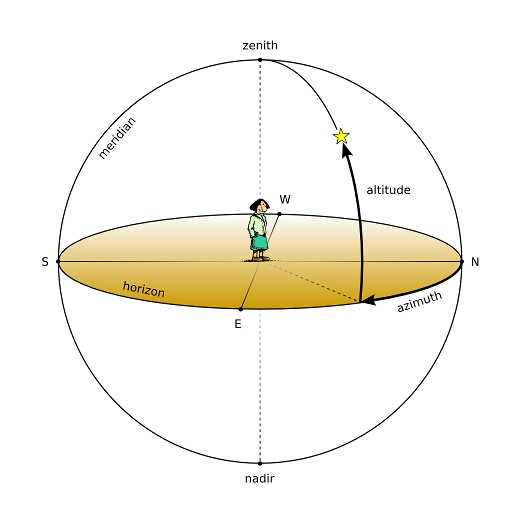
\includegraphics[width=\textwidth]{cs_azi.png}
\caption{Altitude/Azimuth (Horizontal) Coordinate System}
\label{fig:AltAz}
\end{figure}

The 
\indexterm[Coordinate System!Horizontal]{Horizontal Coordinate System} (also called Altitude/Azimuth 
coordinate system) can be used to describe a
direction of view (the \indexterm{azimuth} angle) and an angular
height in the sky (the \indexterm{altitude} angle). The azimuth angle
is measured clockwise round from due north\footnote{In some textbooks
  azimuth is counted from south. There is no global authority to
  decide upon this issue, just be aware of this when you compare
  numbers with other sources.}. Hence North itself is 0$\degree$, East
$90\degree$, Southwest is $225\degree$ and so on.  The altitude angle
is measured up from the \indexterm{mathematical horizon}, which is
just halfway between ``straight up'' and ``straight down'', without
regard to the landscape. Looking directly up (at the
\indexterm{zenith}) would be $90\degree$, half way between the zenith
and the horizon is $45\degree$ and so on. The point opposite the
zenith is called the \indexterm{nadir}.

The Altitude/Azimuth coordinate system is attractive in that it is
intuitive -- most people are familiar with azimuth angles from bearings
in the context of navigation, and the altitude angle is something most
people can visualise pretty easily.

However, the altitude/azimuth coordinate system is not suitable for
describing the general position of stars and other objects in the sky --
the altitude and azimuth values for a celestial object change with
time and the location of the observer.

Stellarium can draw grid lines for altitude/azimuth coordinates. Use the \guibutton{0.6}{bt_az_grid.png}
button on the main toolbar to activate this grid, or press the \key{Z} key.

In addition, the \indexterm{cardinal points} can be highlighted using
the \guibutton{0.6}{bt_cardinal.png} button or \key{Q} key.

There are a few great circles with special names which Stellarium can
draw (see section~\ref{sec:gui:view:markings}).
\begin{description}
\item[Meridian] This is a great circle which runs through the North
  Pole towards the zenith and further to the South Pole and nadir.
\item[(Mathematical) Horizon] This is the line exactly 90\degree\ away
  from the zenith.
\item[First Vertical] This is the vertical circle perpendicular to the horizon and which runs from the East
  point through the zenith, down the West point and to the nadir.
\end{description}

\subsection{Right Ascension/Declination Coordinates}
\label{sec:Concepts:Equatorial}

\begin{figure}[ht]
\centering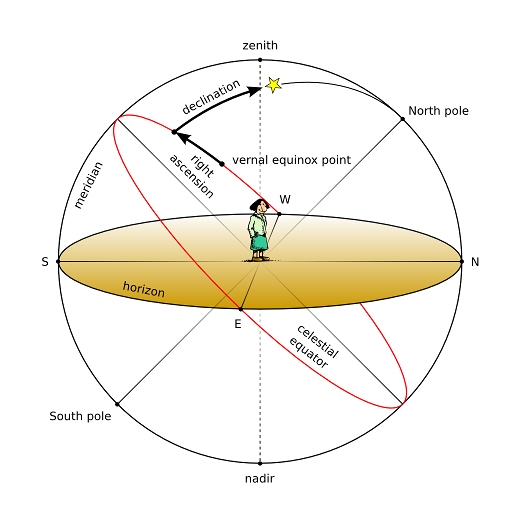
\includegraphics[width=\textwidth]{cs_equ.png}
\caption{Equatorial Coordinates}
\label{fig:EquatorialCoordinates}
\end{figure}

Like the Altitude/Azimuth system, the \indexterm{Right Ascension/Declination}
(RA/Dec) Coordinate System (or \indexterm[Coordinate System!Equatorial]{Equatorial Coordinate System}) uses two angles to describe positions in the sky. These angles are measured from standard points on the celestial
sphere. \indexterm{Right ascension} $\alpha$ and \indexterm{declination} $\delta$ are to the celestial sphere what
longitude and latitude are to terrestrial map makers.

The Northern Celestial Pole has a declination of $\delta=90\degree$, the celestial
equator has a declination of $\delta=0\degree$, and the Southern Celestial Pole has a declination of $\delta=-90\degree$.

%% TODO include Aries in figures
Right ascension is measured as an angle round from the \indexterm{vernal equinox}, a point in the sky
also known as the \indexterm{First Point of Aries} \Aries, in the same way that
longitude is measured around the Earth from
Greenwich. Figure~\ref{fig:EquatorialCoordinates} illustrates RA/Dec
coordinates. The angle $\alpha$ is usually expressed as time with
minute and seconds, with 15\degree\ equaling one hour.

Unlike Altitude/Azimuth coordinates, RA/Dec coordinates of a star do
not change when the observer changes latitude, and do not change
noticeably over the course of the day due to the rotation of the
Earth.  RA/Dec coordinates are generally used nowadays in star
catalogs such as the Hipparcos catalog.

%% see also confusion between "equinox" and "epoch" at https://en.wikipedia.org/wiki/Talk:Epoch_(astronomy)#Epoch_and_Equinox
However, the story is complicated a little by \indexterm{precession}
(section~\ref{sec:Concepts:Precession}) and \indexterm{parallax}
(section~\ref{sec:Concepts:Parallax}). Precession causes a slow drift
of the coordinates almost parallel to the \indexterm{ecliptic},
and therefore star catalogs always have to specify their \indexterm{equinox} of
validity.

Current catalogs and atlases use coordinates for the
\indexterm{standard epoch} J2000.0. The currently best defined
coordinate system, the International Celestial Reference Frame
(\indexterm{ICRF}), is one particular version described in detail in
the astronomical literature \citep{ESAA:2013}. Other catalogs with data
referring to ``J2000.0'' may have to be slightly adjusted (usually in
sub-arcsecond rotations) to match the ICRF coordinate system (short ICRS).

Stars close to the \indexterm[pole, celestial]{celestial poles} are
permanently visible above the horizon and thus called
\indexterm{circumpolar}.  Those stars have observable
\indexterm[culmination, upper]{upper} and \indexterm[culmination,
  lower]{lower culminations} when they pass the meridian arc spanning
from the celestial pole over the zenith to the opposite point on the
horizon, or from the celestial pole to the horizon below,
respectively.

Those circumpolar stars which show their upper culmination between
\indexterm[pole, celestial]{pole} and \indexterm{zenith} also have
limits in \indexterm{azimuth} which they can reach in their daily course,
\newFeature{0.21.2} the points of \indexterm[digression,
  greatest]{greatest digression}. At these points they move vertically
upwards (in the east) or downwards (in the west), respectively.

Stellarium can draw grid lines for equatorial coordinates. Use the
button \guibutton{0.6}{bt_eq_grid.png} on the main toolbar to activate
this grid, or press the \key{E} key to draw the equatorial grid for
the simulation time. The Markings dialog (\ref{sec:gui:view:markings})
allows you to set also the grid for J2000.0 standard coordinates.

There are again a few great circles with special names which
Stellarium can draw in addition, both for simulation time and for
J2000.0 (see section~\ref{sec:gui:view:markings}).
\begin{description}
\item[Celestial Equator] the line directly above the Earth's (or more
  generally, the observer's planet's) equator.
\item[Colures] These are lines similar to meridian and first vertical
  in the azimuthal system. The \indexterm[Colure!Equinoctial]{Equinoctial Colure} runs from the
  North Celestial Pole NCP through the First Point of Aries \Aries,
  South Celestial Pole SCP and First Point of Libra \Libra, while the
  \indexterm[Colure!Solstitial]{Solstitial Colure} runs from the NCP through \indexterm{First Point of
  Cancer} \Cancer, SCP and \indexterm{First Point of Capricorn} \Capricorn.
\end{description}

In case you are observing from another celestial object, the
equatorial coordinates use a system similar to the one referring to
the Earth-based coordinates, but parallel to the planet's rotational
axis.

\subsection{Fixed Equatorial Coordinates}
\label{sec:Concepts:FixedEquatorial}
\index{Coordinate System!Fixed Equatorial}

The celestial sphere with its stars and other objects located in
equatorial coordinates seems to rotate around the celestial polar
axis. When observing with a telescope, it proved useful to mount the
instrument on an axis which is aimed to be parallel to the earth's
axis, i.e., points to the celestial pole. In this case, after setting
the objects's declination, it is enough to move the telescope around
this polar axis to track its course over time and keep the object in
the field of view. We can describe the \indexterm[[Coordinate
    System!Fixed Equatorial]{Fixed Equatorial Coordinate System} as an
  intermediate coordinate system which uses the same equator and
  declination as the equatorial system, but does not rotate as time
  goes by. The longitudinal coordinate is counted in hours from the
  meridian towards the west and is aptly named \indexterm{Hour
    Angle}. A star which has passed the meridian will reach hour angle
  of 1~hour one sidereal hour later.

Stellarium can display \newFeature{0.22.2} the fixed equatorial
coordinates in the Markings dialog (\ref{sec:gui:view:markings}).


\subsection{Ecliptical Coordinates}
\label{sec:Concepts:Ecliptical}
\index{Coordinate System!Ecliptical}

The Earth's orbit around the Sun, i.e., the \indexterm{ecliptic},
defines the ``equatorial line'' of this coordinate system, which is traditionally used when computing the coordinates for planets because of their close proximity to this line.

The zero point of \indexterm{ecliptical longitude} $\lambda$ is the
same as for equatorial coordinates (\Aries), and the \indexterm{ecliptical
  latitude} $\beta$ is counted positive towards the
\indexterm{Northern Ecliptical Pole} NEP in the constellation of
Draco.

Moon and Sun (and to a much lesser extent, the other planets) pull on
the equatorial bulge and try to put Earth's axis normal to its orbital
plane. Earth acts like a spinning top and evades this pull in a
sideways motion, so that Earth's axis seems to describe a small circle
over a period of almost 26.000 years (see section~\ref{sec:Concepts:Precession}). 

In addition, \indexterm[obliquity, ecliptic]{ecliptic obliquity} against the equatorial coordinates,
which mirrors the Earth's axial tilt, slowly changes.

Therefore, also for ecliptical coordinates is is required to specify
which date (epoch) the coordinates refer to.  Stellarium can draw grids
for two epochs. Use the \key{,} key to draw the \indexterm{ecliptic}
for the simulation time. The Markings dialog
(\ref{sec:gui:view:markings}) allows you to also show a line for epoch
J2000.0 and grids for the ecliptical coordinates for current epoch and
epoch J2000.0. You can assign your own shortcut keys
(section~\ref{sec:gui:help:hotkeys}) if you frequently operate with
these coordinates.

Since version 0.14.0 Stellarium can very accurately show the motions
between the coordinate systems~\citep{2011AA:Vondrak, 2012AA:Vondrak}, and it is quite
interesting to follow these motions for several millennia. To support
such demonstrations, Stellarium can also draw the
\indexterm{precession circles} between celestial and ecliptical poles
(activate them in the Markings dialog (\ref{sec:gui:view:markings}).
However, these circles are simply plotted centered on the instantaneous
ecliptic pole by the instantaneous value of obliquity. 
If you observe long enough, you will
see that these circles vary in size, reflecting the changes in
ecliptic \indexterm[obliquity, ecliptic]{obliquity}. The real track of where Earth's axis is pointing forms an open helical loop.

The inner planets are best observed when their apparent distance from
the Sun, or \indexterm{elongation} reaches a maximum. Unfortunately
there are two definitions for elongation, though:
\begin{description}
\item[$\psi$] angular distance on the sphere. This is today the most widely used definition.
\item[$\Delta\lambda_{\text{\Sun}}$] difference between solar and the
  object's ecliptical longitude.\newFeature{0.21.2} The advantage of using this
  definition is that we can easily read \indexterm{opposition}
  ($\Delta\lambda_{\text{\Sun}}=180^\circ$) and \indexterm{conjunction}
  ($\Delta\lambda_{\text{\Sun}}=0^\circ$). We can also see whether we have
  \indexterm[elongation, eastern]{eastern elongation} ($\Delta\lambda_{\text{\Sun}}>0$) where the planet is visible in the evening sky, or
  \indexterm[elongation, western]{western elongation} ($\Delta\lambda_{\text{\Sun}}<0$) where the planet is visible in the morning sky.
  For the inner planets Mercury and Venus
  we further discern \indexterm[conjunction, superior]{superior
    conjunction}, when the planet is ``above'', or behind, the Sun,
  and \indexterm[conjunction, inferior]{inferior conjunction}, when
  the planet is ``below'', or closer than, the Sun.
\end{description}


Many of the minor bodies are best observed around the times of their
opposition.  Stellarium can display a great circle in the ecliptical
coordinates which runs through the ecliptic poles and through the Sun,
thereby allowing to estimate opposition and conjunction. Activate
display of this \indexterm{Opposition/Conjunction Line} in the Markings dialog
(Labeled ``O./C. longitude''; \ref{sec:gui:view:markings}). 
The Markings dialog also provides the possibility to visualize the \indexterm{antisolar point},
which lies opposite of the Sun, on the intersection of the ecliptic and the O/C line.

Another interesting aspect of planets is their \indexterm{quadrature}
from the Sun. \newFeature{0.22.3} Here their angular distance is $90^\circ$.  You can
activate display of the quadrature circle in the Markings dialog
(\ref{sec:gui:view:markings}).

It is interesting to note that star catalogs before \name[Tycho]{Brahe}'s 
(1546--1601), most notably the one in \name{Ptolemy}'s
\indexterm{Almagest}, used ecliptical coordinates. The reason is
simple: it was known since \name{Hipparchus} that stellar coordinates
slowly move along the ecliptic through \indexterm{precession}, and the
correction to coordinates of a date of interest was a simple addition
of a linear correction to the ecliptical longitude in the
catalog. Changes of ecliptic obliquity were discovered much later.

\subsection{Galactic Coordinates}
\label{sec:Concepts:Galactic}

The Milky Way appears to run along a great circle over the sky,
mirroring the fact that the Sun is a star in it. Coordinates for
non-stellar objects which belong to the Milky Way like
\indexterm{pulsars} or \indexterm{planetary nebulae} are often mapped
in \indexterm[Coordinate System!Galactic]{Galactic Coordinates}, 
where \indexterm{galactic longitude} $l$ and 
\indexterm{galactic latitude} $b$ are usually given in decimal
degrees. Here, the zero point of galactic longitudes lies in the
Galactic Center.

Stellarium can also draw a galactic grid and the galactic equator by
activating the respective options in the Markings dialog (see
section~\ref{sec:gui:view:markings}). You can assign a keyboard
shortcut if you frequently use these coordinates
(see~\ref{sec:gui:help:hotkeys}).


\subsection{Planet Coordinates}
\label{sec:Concepts:PlanetCoordinates}

The larger objects in the Solar system are described as spheroids,
sometimes flattened into slightly ellipsoid shape.

Just like the Prime Meridian on Earth has been defined to run through
Greenwich Observatory, each such object in the Solar system for which
any kind of rotation has been detected has a prime meridian defined by
the IAU Working Group on Cartographic Coordinates and Rotational
Elements (WGCCRE). On a rocky planet this is usually defined by some
surface feature like a crater. For the Moon, it has traditionally been
the center of the Lunar disk. For the gas giant planets with
ever-changing atmospheric features, there are even several systems of
rotation. Most notably on Jupiter, System~I describes the rotation of
its equatorial area, while System~II describes the mean atmospheric
rotation north of the south component of the north equatorial belt,
and south of the north component of the south equatorial
belt. Official sources prefer to list the rotation of the magnetic
fields (System~III) for these planets. The most interesting feature on
Jupiter for most observers is the \indexterm{Great Red Spot} (GRS), a
huge storm that has been observed since the 19th, if not even since
the 17th century.

Astronomical almanacs and observing guides often list \emph{transit
  times} when the GRS crosses the center of Jupiter's visible
disk. Stellarium aims to show it at the right place. The storm moves
in longitude, and to adjust for this you can configure its System~II
longitude in the settings, see~\ref{sec:gui:view:sso}.

Like many planet moons, also Earth's Moon shows one side towards its
planet. However, given its elliptical orbit and disturbations by
Earth, Sun and other planets, the Moon seems to nod slightly in
east-west and north-south directions. This motion is called
\indexterm{Libration}. \newFeature{0.21.0} Stellarium gives geocentric
libration in longitude $L$ and latitude $B$, which are the coordinates
of the apparent center of the Lunar disk. Another way to express this
shift is the total angle of libration and the direction into which the
Moon's mean center has been shifted. This angle is given
counterclockwise from the direction of the North pole on the Lunar
disk. The larger this shift is, the better you can observe the
opposite side, which is therefore marked in brackets. If libration is
larger than 3/5/7 degrees, Stellarium shows 1, 2 or 3 exclamation
marks to draw your attention further to this lunar rim. However, you
also need light on this edge.

Another interesting point for which Stellarium gives coordinates is
the sub-solar point $(L_s, B_s)$.

The Selenographic colongitude of the Sun $c_0=450^\circ-L_s$ is given for the
Moon. This helps estimating the terminator \citep{AstronomicalAlgorithms:1998}:
\begin{itemize}
\item The morning terminator is at $360^\circ-c_0$.
\item The evening terminator is at $180^\circ-c_0$.
\item When $c_0=0^\circ$, the Sun rises at selenographic longitude $L=0^\circ$, near First Quarter.
\item When $c_0=90^\circ$, the Sun rises at selenographic longitude $L=270^\circ$, near Full Moon.
\item When $c_0=180^\circ$, the Sun rises at selenographic longitude $L=180^\circ$, near Last Quarter.
\item When $c_0=270^\circ$, the Sun rises at selenographic longitude $L=90^\circ$, near New Moon.
\end{itemize}

$c_0$ is used to compute the Sun's altitude $h$ over a surface point,
e.g.\ a crater on the Moon at position $(\eta, \theta)$, which is
displayed when you select a surface feature.

\begin{equation}
\sin h=\sin B_s \sin\theta + \cos B_s \cos\theta \sin(c_0+\eta)
\end{equation}



\section{Distance}
\label{sec:Concepts:Distance}

As \name[Douglas]{Adams} (1952--2001) pointed out in \citetp{THHG},
\begin{quote}
  Space [\ldots] is big. Really big. You just won't believe how vastly, hugely,
  mind-bogglingly big it is. I mean, you may think it's a long way
  down the road to the chemist, but that's just peanuts to
  space.[p.76]
\end{quote}
%
Astronomers use a variety of units for distance that make sense in the
context of the mind-boggling vastness of space.

\begin{description}
\item[Astronomical Unit (AU)] This is the mean Earth-Sun
  distance. Roughly 150 million kilometers
  ($1.49598 \times 10^8\km$). The AU is used mainly when
  discussing the solar system -- for example the distance of various
  planets from the Sun.
\item[Light year (LY)] A light year is not, as some people believe, a
  measure of time. It is the distance that light travels in a
  year. The speed of light being approximately 300,000 kilometers per
  second means a light year is a very large distance indeed, working
  out at about 9.5 trillion kilometers
  ($9.46073\times10^{12}\km$). Light years are most frequently used
  when describing the distance of stars and galaxies or the sizes of
  large-scale objects like galaxies, nebulae etc.
\item[Parsec (pc)] A parsec is defined as the distance of an object
  that has an annual parallax of 1~second of arc. This equates to
  3.26156 light years ($3.08568\times10^{13}\km$). Parsecs (and derivatives: kiloparsec \kpc, megaparsec \Mpc) are most
  frequently used when describing the distance of stars or the sizes
  of large-scale objects like galaxies, nebulae etc.
\end{description}

\section{Time}
\label{sec:Concepts:Time}

\begin{figure}[ht]
\centering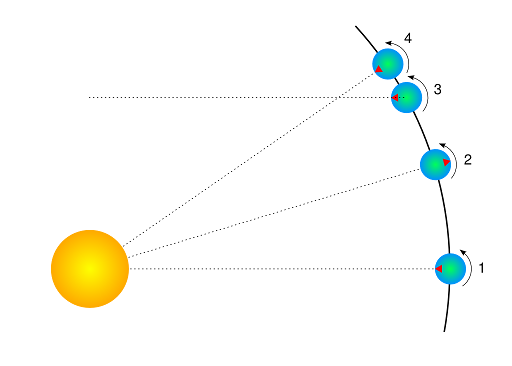
\includegraphics[width=0.95\textwidth]{sidereal_day.png}
\caption{Sidereal day}
\label{fig:SiderealDay}
\end{figure}

The length of a day is defined as the amount of time that it takes for
the Sun to travel from the highest point in the sky at mid-day to the
next high-point on the next day. In astronomy this is called a
\emph{solar day}. The apparent motion of the Sun is caused by the
rotation of the Earth. However, in this time, the Earth not only spins,
it also moves slightly round its orbit. Thus in one solar day the Earth
does not spin exactly $360\degree$ on its axis. Another way to measure day
length is to consider how long it takes for the Earth to rotate exactly
$360\degree$. This is known as one \emph{sidereal day}.

Figure~\ref{fig:SiderealDay} illustrates the motion of the Earth as
seen looking down on the Earth orbiting the Sun. The red triangle on the
Earth represents the location of an observer. The figure shows the Earth
at four times:

\begin{enumerate}
\item
  The Sun is directly overhead - it is mid-day.
\item
  Twelve hours have passed since 1. The Earth has rotated round and the
  observer is on the opposite side of the Earth from the Sun. It is
  mid-night. The Earth has also moved round in its orbit a little.
\item
  The Earth has rotated exactly $360\degree$. Exactly one sidereal day has
  passed since 1.
\item
  It is mid-day again -- exactly one solar day since 1. Note that the
  Earth has rotated more than $360\degree$ since 1.
\end{enumerate}

\noindent It should be noted that in figure~\ref{fig:SiderealDay} the sizes of
the Sun and Earth and not to scale. More importantly, the distance the
Earth moves around its orbit is much exaggerated. The Earth takes a
year to travel round the Sun --
$365\frac{1}{4}$ solar days. The length of a
sidereal day is about 23 hours, 56 minutes and 4 seconds.

\subsection{Sidereal Time}
\label{sec:Concepts:SiderealTime}

It takes exactly one sidereal day for the celestial sphere to make one
revolution in the sky. Astronomers find \indexterm{sidereal time}
useful when observing. This is the Right Ascension which is currently
passing the meridian line, or, equivalent, the \indexterm{Hour Angle}
of the First Point of Aries \Aries.  When visiting observatories, look
out for doctored alarm clocks that have been set to run faster and
show sidereal time!

\subsection{Julian Day Number}
\label{sec:Concepts:JulianDay}

In the 19th century, astronomer \name[John]{Herschel} (1792--1871) introduced the use of
\indexterm{Julian Day} numbers (invented around the time of the Gregorian calendar
reform). This is a simple continuous day count starting on January 1, -4712
(4713 BC). There are no years, months etc., and the integral day
number switches at noon, so during a single night of observation (in
Europe) the date never changes. 

The fractional part of the number is just the fraction of day that has
elapsed since last noon. Given that a day has 86400~seconds, we should
give a JD with 5 decimal places to capture the nearest second.

This causes a problem for modern computers: even a ``double precision
float'' can keep only about 13 decimal places. More than 2.4 million
days have passed, so that e.g. January 1, 2000, 12:00UT is 2451545.0,
which is an accurately storable number with 7 decimal places, but 12:34:56UT is computed as
2451545.02426. A more accurate result would yield
2451545.024259259259... So, for a field where sub-second accuracy
became crucial like spacecraft operations, the \indexterm[Julian Day!Modified]{Modified
  Julian Day} (MJD) has been introduced. It is simply
\begin{equation}
  \label{eq:MJD}
  MJD=JD-2400000.5. 
\end{equation}
This means, days start at midnight, and the (constant, in our era)
decimal places of the ``big numbers'' at the begin of the number have
been traded in for more decimal places at the end. 

Don't put your expectations too high when you see MJD displayed
(section~\ref{sec:gui:date}): Stellarium uses a double-precision
floating point number for JD for internal timekeeping, and Stellarium's
display of MJD is simply computed from it. So you cannot set temporal
increments smaller than a second, and it hardly would make sense to
expect more accuracy from the simulation algorithms.


%\subsubsection{\texorpdfstring{$\mathbf{\Delta T}$}{Delta T}}
\subsection{Delta T}
\label{sec:Concepts:DeltaT}
%% GZ 2016-05-01

Until around 1900, the Earth's rotation was regarded as perfect
standard of time. There were 86400~seconds per mean solar day, and the
accuracy of reproducing time with mechanical clocks only in this time
started to become as good as the Earth's rotation itself.

Astronomers who computed solar eclipses reported in texts from
antiquity wondered about a required time shift which they originally
attributed to a yet-unknown ``secular acceleration of the lunar
motion''. However, it turned out that indeed the gravitational effect
of the Moon which causes the tides also has effects on Earth's
rotation: the tides slowly break Earth's rotational speed. The energy
is also transferred to the Moon, and the acceleration leads to the
Moon slowly moving away from the Earth\footnote{No need to worry, the
  Moon recedes from the Earth only a few centimeters per year as
  measured with the laser reflectors left by the Apollo astronauts in
  the 1970s. In a very far future, however, there will only be annular
  solar eclipses as a consequence!}.

This led to the introduction of a time named Ephemeris Time (ET) with
progresses in the speed of the second in the year 1900, to be used for
positional computation in our solar system, in addition to Greenwich
Mean Time (GMT), from which all zone times and ``civil'' clock times were
derived.

The introduction of atomic clocks in the middle of the 20th century
led to a redefinition of the (temporal) second, which has been
de-coupled from Earth's rotation. This time, the International Atomic
Time TAI\footnote{From the French name \textit{temps atomique international}}, is the basis for Terrestrial Time TT which can be
considered as constantly progressing at constant speed\footnote{We
  don't discuss relativity here. The advanced reader is referred to
  the presentation in the Wikipedia,
  \url{https://en.wikipedia.org/wiki/Delta_T}.}, and is used for
computation of the planetary positions.

Still, people living on Earth prefer to have the mean solar noon
governing the run of day and night. Therefore all forms of civil time
are linked to Coordinated Universal Time UTC. Seconds in UTC and TAI
are of equal length. The slow and irregular divergence between TAI and
UTC is observed by a few standardization institutes.  When necessary,
a leap second can be introduced to the UTC to bring the Earth's
rotation back in sync so that the Mean Sun again culminates at noon.

The difference $\Delta T=TT-UT$ (or ``Delta T'') describes the
temporal offset which amounts already to more than a minute in the 21st
century. There have been many attempts to properly model $\Delta T$,
and Stellarium offers several models you can choose from in the
configuration dialog (see
section~\ref{sec:gui:configuration:time}). ``Espenak and
Meeus (2006)'', is a widely accepted standard. The default, ``Modified Espenak and
Meeus (2006)'', is created to make $\Delta T$ closely in line with observed and predicted
values between the years 2005-2050. But if you are a researcher and want to experiment
with alternative models, you will hopefully like this feature. you can even specify your own data for
$a$, $b$, $c$, $y$ and the secular term for lunar acceleration $n$
(actually $\dot{n}=dn/dt$ in units of
$\mathrm{arcseconds}/\mathrm{century}^2$) if you can model $\Delta T$
according to the formula
\begin{eqnarray}
  \label{eq:DeltaT:custom}
  \Delta T &=& a+ b\cdot u + c \cdot u^2 \, \ \ \text{where}\\
         u &=& \frac{\mathrm{year}-y}{100}
\end{eqnarray}

\subsubsection{List of $\Delta T$ models in Stellarium}
The following list describes sources and a few details about the models for $\Delta T$ implemented in Stellarium.
\begin{description}
\item[Without correction.] Correction is disabled. Use only if you know what you are doing!

\item[Schoch (1931).] This historical formula was obtained by
  \citet{Schoch:1931} and was also used in \citetp{2009ASPC..409..166H}. See for more
  in~\citet{Peters:2010}.   $\dot{n}=-29.68''/\cy^2$.

\item[Clemence (1948).] This empirical equation was published in \citetp{1948AJ.....53..169C}. 
  Valid range of usage: between years 1681 and 1900. $\dot{n}=-22.44''/\cy^2$.

\item[IAU (1952).] This formula is based on a study of post-1650
  observations of the Sun, the Moon and the planets~\citep{1939MNRAS..99..541S} 
  and reproduced in \citetp{AstronomicalFormulaeForCalculators:1988}. %% TODO: Meeus does not give a source!?!?
  It was also adopted in the PC program \program{SunTracker Pro}. Valid range of usage: between years
  1681 and 1936. $\dot{n}=-22.44''/\cy^2$.\index{IAU}

\item[Astronomical Ephemeris (1960).] This is a slightly modified
  version of the IAU~1952 \citep{1939MNRAS..99..541S} formula which was
  adopted in the ``Astronomical Ephemeris''~\citep{ESAE:1961} and in
  the \citetp{Mucke-Meeus:1983}. Valid range of usage: between years
  -500 and 2000. $\dot{n}=-22.44''/\cy^2$.\index{IAU}

\item[Tuckerman (1962, 1964) \& Goldstine (1973).] The famous tables 
\citep{Tuckerman:1962, Tuckerman:1964} list the positions
  of the Sun, the Moon and the planets at 5- and 10-day intervals from
  601 BCE to 1649 CE. The same relation was also implicitly adopted in
  the syzygy tables of \citet{Goldstine:1973}. Valid range of
  usage: between years -600 and 1649.

\item[Muller \& Stephenson (1975).] This equation was published in 
  \citetp{1975grhe.conf..459M}. Valid range of usage:
  between years -1375 and 1975. $\dot{n}=-37.5''/\cy^2$.

\item[Stephenson (1978).] This equation was published in
  \citetp{1978tfer.conf....5S}. $\dot{n}=-30.0''/\cy^2$.

\item[Schmadel \& Zech (1979).] This 12th-order polynomial equation
  (outdated and superseded by \citet{1988AN....309..219S}) was published
  in \citetp{1979AcA....29..101S} as fit through data published
  by \citet{1952AJ.....57..125B}. Valid range of usage: between
  years 1800 and 1975, with meaningless values outside this range. 
  $\dot{n}=-23.8946''/\cy^2$.

\item[Morrison \& Stephenson (1982).] This
  algorithm~\cite{1982ASSL...96..173M} was adopted in 
  \citetp{Bretagnon-Simon:1986} and in the PC planetarium
  program \program{RedShift}. Valid range of usage: between years -4000 and
  2800. $\dot{n}=-26.0''/\cy^2$.

\item[Stephenson \& Morrison (1984).] This formula was published in 
  \citetp{1984RSPTA.313...47S}. Valid range of usage:
  between years -391 and 1600. $\dot{n}=-26.0''/\cy^2$.

\item[Stephenson \& Houlden (1986).] This
  algorithm~\citep{houlden1986supplement} is used in the PC planetarium
  program \program{Guide~7}. Valid range of usage: between years -600 and
  1600.   $\dot{n}=-26.0''/\cy^2$.

\item[Espenak (1987, 1989).] This algorithm was given in 
  \citetp{Espenak:1987} and in 
  \citetp{Espenak:1989}. Valid range of
  usage: between years 1950 and 2100.

\item[Borkowski (1988).] This formula was obtained by
  \citet{1988A&A...205L...8B} from an analysis of 31
  solar eclipse records dating between 2137 BCE and 1715 CE. Valid
  range of usage: between years -2136 and 1715. $\dot{n}=-23.895''/\cy^2$.

\item[Schmadel \& Zech (1988).] This 12th-order polynomial equation
  was published in 
  \citetp{1988AN....309..219S} as data fit through values
  given by \citet{1984RSPTA.313...47S}. Valid range of usage:
  between years 1800 and 1988, with a mean error of less than one
  second, max. error 1.9s, and meaningless values outside this
  range. $\dot{n}=-26.0''/\cy^2$.

\item[Chapront-Touze \& Chapront (1991).] This formula was adopted by
  M. Chapront-Touze \& J. Chapront in the shortened version of the ELP
  2000-85 lunar theory in their \citetp{Chapront-Touze:1991}. The relations are
  based on those of \citet{1984RSPTA.313...47S}, but slightly
  modified to make them compatible with the tidal acceleration
  parameter of $\dot{n}=-23.8946''/\cy^2$ adopted in the ELP 2000-85 lunar
  theory~\citep{1988A&A...190..342C}.

\item[Stephenson \& Morrison (1995).] This equation was published in \citetp{1995RSPTA.351..165S}. 
  Valid range of usage: between years -700 and 1600. $\dot{n}=-26.0''/\cy^2$.

\item[Stephenson (1997).] F. R. Stephenson published this formula in
  his book \citetp{Stephenson:1997}. Valid range of usage: between
  years -500 and 1600. $\dot{n}=-26.0''/\cy^2$.

\item[Meeus (1998) (with Chapront, Chapront-Touze \& Francou (1997)).]
  From \citetp{AstronomicalAlgorithms:1998}, and widely
  used. Table for 1620..2000, and includes a variant of Chapront,
  Chapront-Touze \& Francou (1997) for dates outside 1620..2000. 
  %% TODO: ADD REFERENCE FOR C,C-T,F:1997!
  Valid range of usage: between years -400 and 2150. $\dot{n}=-25.7376''/\cy^2$.

\item[JPL HORIZONS.] The JPL Solar System Dynamics Group of the NASA
  Jet Propulsion Laboratory use this formula in their interactive
  website JPL
  HORIZONS\footnote{\url{https://ssd.jpl.nasa.gov/?horizons}}. Valid
  range of usage: between years -2999 and 1620, with zero values
  outside this range. $\dot{n}=-25.7376''/\cy^2$.

\item[Meeus \& Simons (2000).] This polynome was published in \citetp{2000JBAA..110..323M}. 
  Valid range of usage: between years 1620 and 2000, with zero values outside this
  range. $\dot{n}=-25.7376''/\cy^2$.

\item[Montenbruck \& Pfleger (2000).] The fourth edition of
  \citetp{Montenbruck-Pfleger:2000} provides simple 3rd-order
  polynomial data fits for the recent past. Valid range of usage:
  between years 1825 and 2005, with a typical 1-second accuracy and
  zero values outside this range.

\item[Reingold \& Dershowitz (2002, 2007, 2018).] E. M. Reingold \&
  N. Dershowitz present this polynomial data fit in \citetp{Reingold-Dershowitz:2018} and in their
  \citetp{Reingold-Dershowitz:2007}, \citetp{Reingold-Dershowitz:2002}. It is
  based on \citetp{AstronomicalAlgorithms:1991}.

\item[Morrison \& Stephenson (2004, 2005).] This important solution
  was published in %by L. V. Morrison and F. R. Stephenson in the article
  %``Historical values of the Earth's clock error $\Delta T$ and the
  %calculation of eclipses''~
  \citetp{2004JHA....35..327M} with
  addendum~\citep{2005JHA....36..339M}. Valid range of usage: between
  years -1000 and 2000. $\dot{n}=-26.0''/\cy^2$.

\item[Stephenson, Morrison \& Hohenkerk (2016, 2021).] This important new solution was published 
  %by F. R. Stephenson,  L. V. Morrison and C. Y. Hohenkerk in the article 
  %``Measurement of the Earth’s rotation: 720 BC to AD 2015''~
  in \citetp{StephensonMorrisonHohenkerk:2016}. 
  The solution combines a spline fit to observations (used between the given limits) 
  with a parabolic fit (used as fallback outside the range, but without smooth transitions at the limits, i.e., 
  values for 2016 and later deviate notably from current estimates, and should not be used for dates after 2015).
  The solution was updated in \citetp{StephensonMorrisonHohenkerk:2021}.
  Recommended range of usage: between years -720.0 and 2019.0 $\dot{n}=-25.82''/\cy^2$.
  
\item[Espenak \& Meeus (2006).] This solution by F. Espenak and J. Meeus, based on 
	\citet{2004JHA....35..327M} and a polynomial fit
  through tabulated values for 1600-2000, is used for the NASA Eclipse
  Web Site\footnote{\url{https://eclipse.gsfc.nasa.gov/eclipse.html}}
  and in their \citetp{Espenak-Meeus:2006}. This formula is also used in the
  solar, lunar and planetary ephemeris program \program{SOLEX}. Valid
  range of usage: between years -1999 and
  3000. $\dot{n}=-25.858''/\cy^2$.

\item[Modified Espenak \& Meeus (2006).] This solution\footnote{This solution
  is used by default.} is a modification from Espenak \& Meeus (2006). Two formulae are developed to make $\Delta T$
  closely in line with observed and predicted values by IERS and also connected with original values.
  Valid range of usage: between years -1999 and 3000. $\dot{n}=-25.858''/\cy^2$.

\item[Reijs (2006).] From the Length of Day (LOD; as determined by
  \citet{2004JHA....35..327M}), Victor Reijs
  derived a $\Delta T$ formula by using a Simplex optimization with a
  cosine and square
  function.
  % \footnote{\url{http://www.iol.ie/~geniet/eng/DeltaTeval.htm}}. 
  This is based on a possible periodicity described by
  \citet{2004JHA....35..327M}. Valid range of usage: between
  years -1500 and 1100. $\dot{n}=-26.0''/\cy^2$.

\item[Banjevic (2006).] This solution is based on
  \citet{1984RSPTA.313...47S} and was
  published in \citetp{2006POBeo..80..251B}. Valid range of usage: between
  years -2020 and 1620, with zero values outside this range. 
  $\dot{n}=-26.0''/\cy^2$.

\item[Islam, Sadiq \& Qureshi (2008, 2013).] This solution by
  S. Islam, M. Sadiq and M. S. Qureshi, based on \citet{2000JBAA..110..323M}, was published in 
  \citetp{Islam-Sadiq-Qureshi:2008} and revisited by Sana Islam
  in 2013. Valid range of usage: between years 1620 and 2007, with
  zero values outside this range.

\item[Khalid, Sultana \& Zaidi (2014).] This polynomial approximation with 0.6~seconds 
  of accuracy was published in \citetp{Khalid-Sultana-Zaidi:2014}. 
  Valid range of usage: between years 1620 and 2013, with zero values outside this range.

\item[Henriksson (2017).] \newFeature{0.18.2} A solution which combines Schoch's 1931
  solution (parabolic fit) with a discussion of and correction for relativistic effects.  The author
  claims an accurate fit for solar eclipses probably depicted in artifacts going back to the mid-fourth
  millennium BC.
  Also with this setting, the exact times from his paper \citep{Henriksson:2017} cannot be
  reproduced probably because the author used a different ephemeris, but the phenomena are
  plausibly reproduced.
  Recommended range of usage: between years -4000.0 and 2000.0 $\dot{n}=-30.128''/\cy^2$.

\item[Custom equation of $\Delta T$.] This is the quadratic formula \ref{eq:DeltaT:custom} for
  calculation of $\Delta T$ with coefficients defined by the user.
\end{description}


\section{Angles}
\label{sec:Concepts:Angles}

Astronomers typically use degrees to measure angles. Since many
observations require very precise measurement, the degree is subdivided
into sixty \emph{minutes of arc} also known as \emph{arc-minutes}. Each
minute of arc is further subdivided into sixty \emph{seconds of arc}, or
\emph{arc-seconds}. Thus one degree is equal to 3600 seconds of arc.
Finer grades of precision are usually expressed using the SI prefixes
with arc-seconds, e.g. \emph{milli arc-seconds} (one milli arc-second is
one thousandth of an arc-second).

\subsection{Notation}

Degrees are denoted using the $\degree$ symbol after a number. Minutes of arc are denoted with a~$'$, and seconds of arc are denoted using~$''$. Angles are frequently given in two formats:

\begin{enumerate}
\item
  DMS format --- degrees, minutes and seconds. For example $90\degree15'12''$.
  When more precision is required, the seconds component may include a
  decimal part, for example $90\degree15'12.432''$.
\item
  Decimal degrees, for example $90.2533\degree$
\end{enumerate}

\subsection{Handy Angles}
\label{sec:Concepts:Angles:HandyAngles}
\index{Handy Angles}

Being able to estimate angular distance can be very useful when trying
to find objects from star maps in the sky. One way to do this with a
device called a \indexterm{crossbow}.

%% GZ TODO: Add figure of my crossbow!

Crossbows are a nice way get an idea of angular distances, but carrying
one about is a little cumbersome. A more convenient alternative is to
hold up an object such as a pencil at arm's length. If you know the
length of the pencil, $d$, and the distance of it from your eye, $D$, you
can calculate its angular size, $\theta$ using this formula:

\begin{equation}
\label{eq:handyAngle}
\theta=2 \cdot \arctan{\left(\frac{d}{2 \cdot D}\right) }
\end{equation}


\noindent Another, more handy (ahem!) method is to use the size of your hand at
arm's length:

\begin{description}
\item[Tip of little finger] About 1\degree 
\item[Middle three fingers] About 4\degree 
\item[Across the knuckles of the fist] About 10\degree 
\item[Open hand] About 18\degree
\end{description}

Using your hand in this way is not very precise, but it's close enough
to give you some way to translate an idea like ``Mars will be
$45\degree$ above the southeastern horizon at 21:30''. Of course,
there are variations from person to person, but the variation is
compensated for somewhat by the fact that people with long arms tend
to have larger hands. In exercise~\ref{sec:Exercises:handyAngles} you
will work out your own ``handy angles''.



\section{The Magnitude Scale}
\label{sec:Concepts:Magnitudes}


When astronomers talk about magnitude, they are referring to the
brightness of an object. How bright an object appears to be depends on
how much light it is giving out and how far it is from the observer.
Astronomers separate these factors by using two measures: \indexterm{absolute
magnitude} (Mag or $M$) which is a measure of how much light is being
given out by an object, and \indexterm{apparent magnitude} (mag or $m$) which
is how bright something appears to be in the sky.

For example, consider two 100 watt lamps, one which is a few meters
away, and one which is a kilometer away. Both give out the same amount
of light -- they have the same absolute magnitude. However the nearby
lamp seems much brighter -- it has a much greater apparent magnitude.
When astronomers talk about magnitude without specifying whether they
mean apparent or absolute magnitude, they are usually referring to
apparent magnitude.

The magnitude scale has its roots in antiquity. The Greek astronomer
\name{Hipparchus} defined the brightest stars in the sky to be \emph{first
magnitude}, and the dimmest visible to the naked eye to be \emph{sixth
magnitude}. In the 19th century British astronomer \name[Norman]{Pogson} (1829--1891)
quantified the scale more precisely, defining it as a logarithmic scale
where a magnitude~1 object is 100~times as bright as a magnitude~6
object (a difference of five magnitudes). The zero-point of the modern
scale was originally defined as the brightness of the star Vega, however
this was re-defined more formally in 1982 \citep{landolt}. Objects brighter
than Vega are given negative magnitudes.

The absolute magnitude of a star is defined as the magnitude a star
would appear if it were 10 parsecs from the observer.

Table~\ref{tab:Concepts:Magnitudes} lists several objects that may be seen
in the sky, their apparent magnitude and their absolute magnitude where
applicable (only stars have an absolute magnitude value. Planets nor Moon emit light like a star does -- they reflect the light from the Sun).

\begin{table}[htb]
  \centering
  \begin{tabular}{lll}
\toprule
\emph{Object} & $m$ & $M$\\\midrule
The Sun & -27 & 4.8\\
Vega & 0.05 & 0.6\\
Betelgeuse & 0.47 & -7.2\\
Sirius (the brightest star) & -1.5 & 1.4\\
Venus (at brightest) & -4.4 & ---\\
Full Moon (at brightest) & -12.6 & ---\\
\bottomrule
\end{tabular}
  \caption{Magnitudes of a few objects}
  \label{tab:Concepts:Magnitudes}
\end{table}


\section{Luminosity}
\label{sec:Concepts:Luminosity}

\emph{Luminosity} is an expression of the total energy radiated by a
star. It may be measured in watts, however, astronomers tend to use
another expression --- \emph{solar luminosities} where an object with
twice the Sun's luminosity is considered to have two solar luminosities
and so on. Luminosity is related to absolute magnitude.

\section{Precession}
\label{sec:Concepts:Precession}

\begin{figure}[htb]
\centering
\includegraphics[width=\textwidth]{obliquity_ecliptic.png}
\caption{Ecliptic obliquity}
\label{fig:Obliquity}
\end{figure}

\noindent As the Earth orbits the Sun throughout the year, the axis of rotation
(the line running through the rotational poles of the Earth) seems to
point towards the same position on the celestial sphere, as can be
seen in figure~\ref{fig:Obliquity}. The angle between the axis of
rotation and the perpendicular of the orbital plane is called the
\indexterm[obliquity, ecliptic]{obliquity of the ecliptic}. It is currently about
$23\degree27'$ and is the angle between equatorial plane
(\ref{sec:Concepts:Equatorial}) and ecliptical plane
(\ref{sec:Concepts:Ecliptical}).

\begin{figure}[p]
\centering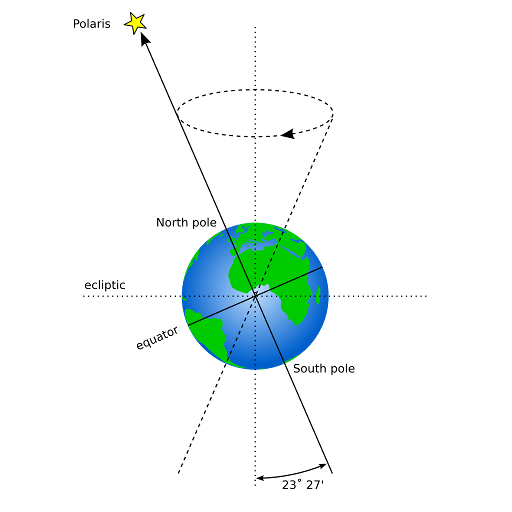
\includegraphics[width=0.75\textwidth]{precession.png}
\caption{Precession}
\label{fig:Precession}
\end{figure}

\begin{figure}[p]
\centering
\ifpdf
\includegraphics[width=\textwidth]{P_BSC-PrecessionShift-Horizon30_85-135_1000BC-0_en}
\else
\includegraphics[width=\textwidth]{P_BSC-PrecessionShift-Horizon30_85-135_1000BC-0_en.png}
\fi
\caption{Precession: Change of rising positions of the stars along the
  eastern horizon from azimuths 85 to 135 degrees, between years 1000
  BC and 0, for latitude $\varphi=30\degree$.}
\label{fig:Precession:AzimuthShift}
\end{figure}




Observed over very long periods of time the direction the axis of
rotation points to does actually change. The angle between the axis of
rotation and the orbital plane stays fairly constant, but the
direction the axis points --- the position of the celestial pole ---
transcribes a figure similar to a circle on the celestial sphere. The motion
is similar to the way in which a gyroscope slowly twists, as
figure~\ref{fig:Precession} illustrates. This process is called
\indexterm{precession}. The circles can be shown in Stellarium: from
the View menu (\key{F4}), tab ``Markings'', switch on ``Precession
Circles'' (\ref{sec:gui:view:markings}).

Precession is a slow process. The axis of rotation twists through a
full $360\degree$ about once every 26,000 years. However, over these
long times other gravitational perturbations (``planetary
precession'') play a role, and what may be thought of as rigid
``precession circle'' can actually only show the instantaneous
(current) state. Over millennia the circle slightly varies.

Precession has some important implications:

\begin{enumerate}
\item RA/Dec coordinates change over time, albeit slowly. Measurements
  of the positions of stars recorded using RA/Dec coordinates must
  also include a date (``equinox'') for those coordinates. Therefore
  the current star catalogues list their objects for the epoch and
  equinox J2000.0.
\item Polaris, the Pole Star, won't stay a good indicator of the
  location of the Northern Celestial Pole. In 14,000 years time
  Polaris will be nearly $47\degree$ away from the celestial pole!
\item The change in declination causes a shift in the rising and
  setting positions of the stars along the
  horizon. Figure~\ref{fig:Precession:AzimuthShift} shows part of the
  horizon for latitude $\varphi=30\degree$ north. For a given year
  (left vertical labels), make a horizontal line to find rising
  azimuth of the bright stars indicated by the twisting
  lines. Depending on where on the celestial sphere a star is located,
  it may appear to move north or south, or be almost stationary for
  several centuries.
\end{enumerate}


\section{Parallax}
\label{sec:Concepts:Parallax}


Parallax is the change of angular position of two stationary points
relative to each other as seen by an observer, due to the motion of said
observer. Or more simply put, it is the apparent shift of an object
against a background due to a change in observer position.

This can be demonstrated by holding one's thumb up at arm's length.
Closing one eye, note the position of the thumb against the background.
After swapping which eye is open (without moving), the thumb appears to
be in a different position against the background.

\subsection{Geocentric and Topocentric Observations}
\label{sec:Concepts:Parallax:Topocentric}

%% Author GZ 2016-01-11

When computing planetary positions was done manually by adding numbers
tabulated in yearly almanacs, computing the Earth's position and, say, the
position of a minor planet was usually good enough to find the object
in the sky. In both cases, the exact numbers refer to the
gravitational centers of the respective bodies. However, we are
sitting on Earth's surface, so the observed planet will be seen in a
slightly shifted location. The amount for objects in the inner solar
system is usually just a few arc-seconds and is mostly negligible when we
just want to find an object. But it makes a difference when it comes
to observations of stellar occultations by planets or asteroids. Such
a body may measure only a few tens of kilometers, and the shadow track
which it leaves on Earth's surface is of approximately the same
size.\footnote{Unfortunately Stellarium (as of v0.15.0) is not accurate
  enough to reliably compute such occultations. Even a deviation of
  0.5 arc-seconds is too much here.}

A much closer and bigger object is the Moon, which can also occult
stars. It can even occult the one big star we call the Sun: this is a
solar eclipse. And here it makes a huge difference where on the planet
you are located. 

If you are interested in astronomical computing, you may still be
interested in geocentric numerical results. From the Settings panel
(\key{F2}), tab ``Tools'', there is a checkbox for ``Topocentric
Coordinates''. Switch it off to put yourself into the center of the
planet you are located.

\subsection{Stellar Parallax}
\label{sec:Concepts:StellarParallax}

\begin{figure}[tb]
\centering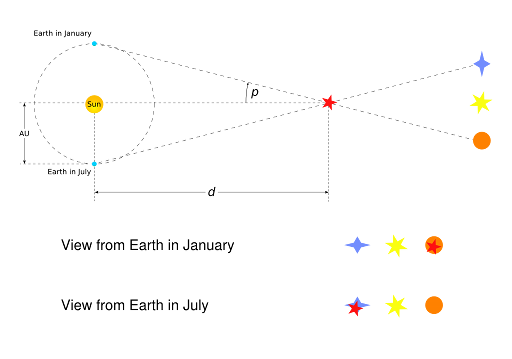
\includegraphics[width=0.75\textwidth,trim=5 40 5 25,clip]{parallax.png}
\caption{Stellar Parallax}
\label{fig:Parallax}
\end{figure}

A similar thing happens due to the Earth's motion around the Sun. Nearby
stars appear to move against more distant background stars, as
illustrated in figure~\ref{fig:Parallax}.
The movement of nearby stars against the background is called
\indexterm{stellar parallax}, or \indexterm{annual parallax}.

Since we know the radius of the Earth's orbit around the
Sun from other methods, we can use simple geometry to calculate the
distance of the nearby star if we measure annual parallax.

As can be seen from figure~\ref{fig:Parallax}, the annual
parallax $p$ is half the angular distance between the apparent positions
of the nearby star. The distance of the nearby object is $d$. Astronomers
use a unit of distance called the parsec ($\pc$) which is defined as the
distance at which a nearby star has $p=1''$.

Even the nearest stars exhibit very small movement due to
parallax. The closest star to the Earth other than the Sun is Proxima
Centauri. It has an annual parallax of $0.77199''$, corresponding to a
distance of $1.295\pc$ (4.22 light years).

Even with the most sensitive instruments for measuring the positions of
the stars it is only possible to use parallax to determine the distance
of stars up to about 1,600 light years from the Earth, after which the
annual parallax is so small it cannot be measured accurately enough.

In Stellarium, the annual parallax can be listed in the object information for stars
when available. It is not accounted for in the positional calculations.

\section{Aberration of Light}
\label{sec:Concepts:Aberration}

\newFeature{0.21.2} When you are standing under a rainy but
windless sky with an umbrella placed vertically over your head, your
feet will not be hit by raindrops. But when you are walking, raindrops
which just missed the umbrella may hit your feet. Relative to your
umbrella and feet, it seems that the raindrops are coming not quite
vertically from above, but inclined from the direction you are heading
into, and therefore you tilt the umbrella slightly forward to fend off
the raindrops from your feet.

Light propagates very fast compared to the motion of the planets, but
still with a finite velocity. Therefore, just like the raindrops
mentioned above, light from all celestial objects seem to come in from
a position slightly distorted towards the point in space the observer
is heading to.

In search for stellar parallax (see section \ref{sec:Concepts:StellarParallax}),
this effect of the \indexterm{aberration of light} was fortuitously
discovered and then explained by \name[James]{Bradley} (1693--1762) in
1725. This was also the final proof for Earth's movement around the
Sun. For an observer on the moving Earth, the apparent deviation of a
star from the mean coordinates can reach $20.4"$. As the months pass,
Earth is changing its direction along its orbit, and so the light
distortion also changes, i.e., the direction towards the object moves
against the fixed coordinate axes. The effect is significant when we
want to compute, for example, stellar occultations by the Moon.

In Stellarium, you can observe a slight annual wobble in all objects'
positions against the fixed celestial grids. Just enable the
equatorial grid, zoom in and run through the months. You can also
exaggerate the aberration effect upto $5\times$ to make it more
apparent. \footnote{Exaggerating even more causes graphics defects and
  has been disabled for now.}

\section{Proper Motion}
\label{sec:Concepts:ProperMotion}

\indexterm[proper motion]{Proper motion} is the change in the position of a star over time as a
result of its motion through space relative to the Sun. It does not
include the apparent shift in position of star due to annular parallax.
The star exhibiting the greatest proper motion is \indexterm{Barnard's Star} which
moves more than ten seconds of arc per year.

If you want to simulate the effect of proper motion with Stellarium,
put the map into equatorial view mode, switch off ground and cardinal
marks, and set some high time lapse speed. You will see a few stars
change their locations quite soon, those are usually stars in our
galactic neighbourhood (see section~\ref{sec:Exercises:ProperMotion}).

Note however some limitations:
\begin{enumerate}
\item Stellarium will stop at $\pm 100.000$ years. This limit may be
  still suitable for most stellar locations. The planetary locations
  are not trustworthy outside of a much narrower temporal window (see
  section~\ref{ch:Accuracy}). You cannot simulate the sky over the
  dinosaurs or such things.
\item Proper motion is only modeled by linear components. True 3D
  motion in space requires more computation, which would slow down the
  program.
\item Double stars are listed in catalogs as two individual stars with
  their current proper motion which consists of a common spatial motion and the 
  orbital motion around their common center of gravity. However, their orbital
  motion around each other is not modelled in Stellarium.  They may be seen flying 
  apart, which is of course not realistic.
\end{enumerate}

%%% Local Variables: 
%%% mode: latex
%%% TeX-PDF-mode: t
%%% TeX-master: "guide"
%%% End: 
